\documentclass[xcolor=dvipsnames
              %,handout
              ]{beamer} 

\usetheme{Madrid} 
%\setbeamertemplate{blocks}[shadow=false] 
\setbeamertemplate{navigation symbols}{} 
\setbeamertemplate{items}[square]
\setbeamertemplate{sections/subsections in toc}[square]

\definecolor{myblueend}{rgb}{0.058,0.132,0.42}
\definecolor{mybluemiddle}{rgb}{0.31,0.45,0.64}
\definecolor{mybluestart}{rgb}{0.17,0.28,0.48}
\definecolor{mygreen}{rgb}{0,0.7,0}
\definecolor{mylightgreen}{rgb}{0.7,1,0.7}
\definecolor{mylightblue}{rgb}{0.7,0.7,1}
\definecolor{mylightblack}{rgb}{0.7,0.7,0.7}
\definecolor{mylightred}{rgb}{1,0.7,0.7}
\definecolor{oproverblue}{RGB}{12,83,144}
\definecolor{oproveryellow}{RGB}{255,156,55}
\definecolor{mydarkgreen}{rgb}{0.17,0.48,0.28}
\definecolor{mydarkred}{rgb}{0.48,0.28,0.17}
\definecolor{grey}{rgb}{0.7,0.7,0.7}
\definecolor{darkgrey}{rgb}{0.5,0.5,0.5}

%\setbeamercolor{palette primary}{fg=white,bg=mybluestart}
%\setbeamercolor{palette secondary}{fg=white,bg=mybluestart}
%\setbeamercolor{palette tertiary}{fg=white,bg=mybluestart}
%\setbeamercolor{palette quaternary}{fg=white,bg=mybluestart}
\setbeamercolor{palette primary}{fg=white,bg=oproverblue}
\setbeamercolor{palette secondary}{fg=white,bg=oproverblue}
\setbeamercolor{palette tertiary}{fg=white,bg=oproverblue}
\setbeamercolor{palette quaternary}{fg=white,bg=oproverblue}
\setbeamercolor{titlelike}{parent=palette quaternary}

\setbeamercolor{item}{fg=oproverblue}
\setbeamercolor{block title}{fg=white,bg=oproverblue}
\setbeamercolor{block title example}{fg=white,bg=oproveryellow}
%\setbeamercolor{block title alert}{fg=white,bg=mydarkred}

\usefonttheme{serif}

%%
%% TOOLS
%% 
\newcommand{\opensmt}{{\sc OpenSMT}\xspace}
\newcommand{\yices}{{\sc Yices}\xspace}
\newcommand{\mathsat}{{\sc MathSAT}\xspace}
\newcommand{\cvcfour}{{\sc CVC4}\xspace}
\newcommand{\zthree}{{\sc Z3}\xspace}
\newcommand{\boolector}{{\sc Boolector}\xspace}
\newcommand{\verit}{{\sc veriT}\xspace}
\newcommand{\stp}{{\sc STP}\xspace}
\newcommand{\minisat}{{\sc MiniSAT}\xspace}
%%
%% BOOLEAN OPERATORS
%%
\newcommand{\swedge}{\,\wedge\,}
\newcommand{\svee}{\,\vee\,}
\newcommand{\impl}{\,\rightarrow\,}
%%
%% SMTLIB LOGICS
%% 
\newcommand{\Idl}{\ensuremath{\mathcal{IDL}}\xspace}
\newcommand{\Rdl}{\ensuremath{\mathcal{RDL}}\xspace}
\newcommand{\Uf}{\ensuremath{\mathcal{UF}}\xspace}
\newcommand{\Lia}{\ensuremath{\mathcal{LIA}}\xspace}
\newcommand{\Lra}{\ensuremath{\mathcal{LRA}}\xspace}
\newcommand{\Arrays}{\ensuremath{\mathcal{A}}\xspace}
\newcommand{\Bitvectors}{\ensuremath{\mathcal{BV}}\xspace}
\newcommand{\T}{\ensuremath{\mathcal{T}}\xspace}
\newcommand{\B}{\ensuremath{\mathcal{B}}\xspace}
%%
%% SETS
%%
\newcommand{\Int}{\ensuremath{\mathbb{Z}}\xspace}
\newcommand{\Rat}{\ensuremath{\mathbb{Q}}\xspace}
\newcommand{\Rea}{\ensuremath{\mathbb{R}}\xspace}
\newcommand{\Boo}{\ensuremath{\mathbb{B}}\xspace}
%%
%% SORTS
%%
\newcommand{\SInt}{{\tt Int}\xspace}
\newcommand{\SRea}{{\tt Real}\xspace}
\newcommand{\SBoo}{{\tt Bool}\xspace}
\newcommand{\SBv}[1]{{\tt BV}$_{[#1]}$\xspace}
%%
%% SMT specific
%%
\newcommand{\tconflict}{\T-conflict\xspace}
\newcommand{\tconflicts}{\T-conflicts\xspace}
\newcommand{\tterm}{\T-term\xspace}
\newcommand{\tterms}{\T-terms\xspace}
\newcommand{\tatom}{\T-atom\xspace}
\newcommand{\tatoms}{\T-atoms\xspace}
\newcommand{\tlit}{\T-literal\xspace}
\newcommand{\tlits}{\T-literals\xspace}
\newcommand{\tformula}{\T-formula\xspace}
\newcommand{\batom}{\B-atom\xspace}
\newcommand{\batoms}{\B-atoms\xspace}
\newcommand{\blit}{\B-literal\xspace}
\newcommand{\blits}{\B-literals\xspace}
\newcommand{\babst}[1]{#1^{\B}}
\newcommand{\tsolver}{\T-solver\xspace}
\newcommand{\tsolvers}{\T-solvers\xspace}
%%
%% SAT specific
%%
\newcommand{\dec}[2]{\stackrel{\textcolor{oproveryellow}{#2}}{#1}}
%%
%% BIT-VECTORS
%%
\newcommand{\w}[2]{\ensuremath{#1_{[#2]}}}
\newcommand{\band}{\,{\bf AND}\,}
\newcommand{\bor}{\,{\bf OR}\,}
\newcommand{\bnot}{{\bf NOT}\,}
\newcommand{\bitandsymb}{\,\, {\bf AND}}
\newcommand{\bit}[2]{#1\ensuremath{^#2}}
%%
%% IDL graphs
%%
\newcommand{\idlnode}[2]{\frac{#1}{#2}}
%%
%% LRA Solver
%%
\newcommand{\bas}{\ensuremath{\mathcal{B}}\xspace}
\newcommand{\nonbas}{\ensuremath{\mathcal{N}}\xspace}
%%
%% MISC
%%
\newcommand{\Lbrack}{\ensuremath{[\mspace{-3mu}[}}
\newcommand{\Rbrack}{\ensuremath{]\mspace{-3mu}]}}
\newcommand{\inter}[1]{\ensuremath{\Lbrack #1 \Rbrack}}
\newcommand{\COMMENT}[1]{}
\newcommand{\hl}[1]{\colorbox{oproveryellow}{\bf #1}}
\newcommand{\colfou}[1]{\textcolor{grey}{#1}}
\newcommand{\formulae}{formul\ae\xspace}
\newcommand{\smtsolvers}{SMT-solvers\xspace}
\newcommand{\smtsolver}{SMT-solver\xspace}
\newcommand{\satsolvers}{SAT-solvers\xspace}
\newcommand{\satsolver}{SAT-solver\xspace}
\newcommand{\bitvectors}{Bit-Vectors\xspace}
\newcommand{\bitvector}{Bit-Vector\xspace}
\newcommand{\colone}[1]{\textcolor{red}{#1}}
\newcommand{\coltwo}[1]{\textcolor{mygreen}{#1}}
\newcommand{\coloneat}[2]{\textcolor<#2>{red}{#1}}
\newcommand{\coltwoat}[2]{\textcolor<#2>{mygreen}{#1}}
\newcommand{\colfouat}[2]{\textcolor<#2>{grey}{#1}}
\newcommand{\claset}{\mathcal{C}}
\newcommand{\ra}[1]{\renewcommand{\arraystretch}{#1}}

\usepackage{epsfig}
\usepackage{graphicx}
\usepackage{color}
\usepackage{amstext}
\usepackage{amssymb}
\usepackage{amsfonts}
\usepackage{amsmath}
\usepackage{amsthm}
\usepackage{xspace}
\usepackage{multirow}
\usepackage{tabularx,colortbl}
\usepackage{alltt}
\usepackage{bussproofs}
\usepackage{algorithm2e}
\usepackage{datetime}
\usepackage{tikz}


\title[\opensmt]{Satisfiability Modulo Theories\\ Lecture 9 - Extending \opensmt for fun and profit$^*$\\ {\tiny (slides revision: \today, \currenttime)}}
\author[R. Bruttomesso]{\large Roberto Bruttomesso}
\date{22 Dicembre 2011}
\institute[SMT]{\large Seminario di Logica Matematica \\ (Corso Prof. Silvio Ghilardi)}
\logo{ \vspace{-6pt} \includegraphics[scale=0.15]{imgs/logo-ita.png} }

\begin{document}

\frame{\titlepage}

\begin{frame}
  \frametitle{Outline}
  \tableofcontents
\end{frame}

\section{A simple logic}
\begin{frame}
  \frametitle{A simple logic}

  For this tutorial we use a theory that we call ``simple order'' (\So)
  \vfill
  Atoms of this theory are of the form
  $$
    x \leq y
  $$
  but $\leq$ it is just a symbol to intend ``$x$ is before $y$''
  \vfill
  A set of constraints is unsatisfiable iff there is a cycle 
  $$x \leq y,\ y \leq z,\ \ldots,\ w \leq x$$  
  \vfill
  A model is therefore is any ``acyclic'' set of constraints
  \vfill

  \begin{columns}

    \begin{column}{.3\textwidth}

      \begin{overlayarea}{.3\textwidth}{40pt}

	\only<1|handout:0>{
	$x \leq y$ \\
	$y \leq z$ \\
	$z \leq x$
	}
	\only<2>{
	$x \leq y$ \\
	$y \leq z$ \\
	$x \leq z$
	}

      \end{overlayarea}
      
    \end{column}
    
    \begin{column}{.4\textwidth}

      \begin{overlayarea}{.4\textwidth}{40pt}
      \only<1|handout:0>{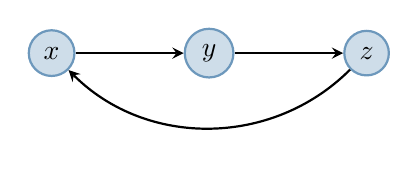
\begin{tikzpicture}[auto]

%
% Styles
%
\tikzstyle{vertex} = [circle,draw=oproverblue!60,fill=oproverblue!20,thick]
\tikzstyle{edge}   = [->,>=stealth,thick]

\node[vertex] (x) at ( 0, 0)  {$x$};
\node[vertex] (y) at ( 2, 0)  {$y$};
\node[vertex] (z) at ( 4, 0)  {$z$};

\draw[edge] (x) -- (y);
\draw[edge] (y) -- (z);
\draw[edge] (z) to [out=225,in=-45] (x);

\end{tikzpicture}
}
      \only<2>{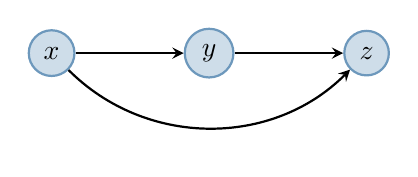
\begin{tikzpicture}[auto]

%
% Styles
%
\tikzstyle{vertex} = [circle,draw=oproverblue!60,fill=oproverblue!20,thick]
\tikzstyle{edge}   = [->,>=stealth,thick]

\node[vertex] (x) at ( 0, 0)  {$x$};
\node[vertex] (y) at ( 2, 0)  {$y$};
\node[vertex] (z) at ( 4, 0)  {$z$};

\draw[edge] (x) -- (y);
\draw[edge] (y) -- (z);
\draw[edge] (x) to [out=-45,in=225] (z);

\end{tikzpicture}
}
      \end{overlayarea}
      
    \end{column}

    \begin{column}{.2\textwidth}

      \only<1|handout:0>{unsat}\only<2>{sat}

    \end{column}

  \end{columns}

\end{frame}


\section{Phase 0 - Compiling \opensmt}
\begin{frame}[fragile]
  \frametitle{Phase 0 - Compiling \opensmt for the first time}

  \begin{verbatim}

    $ autoreconf --install [--force]


    $ mkdir debug


    $ cd debug


    debug $ ../configure --disable-optimization 
                         [--with-gmp=/opt/local]


    debug $ make [-j4]
    debug $ cd ..

  \end{verbatim}

\end{frame}


\section{Phase 1 - Setting up files and directories}
\begin{frame}[fragile]
  \frametitle{Phase 1 - Setting up files and directories}

  \begin{enumerate}[1.]

    \item Create a new directory for \So-solver

    \begin{enumerate}[a.]

      \item \verb|$ cd src/tsolvers|

      \item \verb|src/tsolvers $ cp -r emptysolver sosolver|

    \end{enumerate}

    \vfill\pause

    \item Rename files

    \begin{enumerate}[a.]

      \item \verb|src/tsolvers $ cd sosolver|

      \item \verb|src/tsolvers/sosolver $ mv EmptySolver.h SOSolver.h|

      \item \verb|src/tsolvers/sosolver $ mv EmptySolver.C SOSolver.C|

    \end{enumerate}

    \vfill\pause

    \item Adjust Makefile.am

    \begin{enumerate}[a.]

      \item \verb|src/tsolvers/sosolver $ rm Makefile.in|

      \item \verb|src/tsolvers/sosolver $ vim Makefile.am|

      \item Find-replace ``\verb|empty|'' with ``\verb|so|'' and 
            ``\verb|Empty|'' with ``\verb|SO|''
	    in the file (\verb|:%s/empty/so/g| and \verb|:%s/Empty/SO/g| with vim)

    \end{enumerate}

  \end{enumerate}

\end{frame}

\begin{frame}[fragile]
  \frametitle{Phase 1 - Setting up files and directories}

  \begin{enumerate}[4.]

    \item Adjust source files

    \begin{enumerate}[a.]

      \item \verb|src/tsolvers/sosolver $ vim SOSolver.h|

      \item Find-replace ``\verb|EMPTY|'' with ``\verb|SO|''
            (\verb|:%s/EMPTY/SO/g| with vim)

      \item Find-replace ``\verb|Empty|'' with ``\verb|SO|''
            (\verb|:%s/Empty/SO/g| with vim)

      \item \verb|src/tsolvers/sosolver $ vim SOSolver.C|

      \item Find-replace ``\verb|Empty|'' with ``\verb|SO|''
            (\verb|:%s/Empty/SO/g| with vim)

    \end{enumerate}

  \end{enumerate}

  \vfill\pause

  \begin{enumerate}[5.]

    \item Adjust \verb|../Makefile.am|

    \begin{enumerate}[a.]

      \item \verb|src/tsolvers/sosolver $ cd ..|

      \item \verb|src/tsolvers $ vim Makefile.am|

      \item Add \verb|sosolver| in \verb|SUBDIR| list

      \item Add \verb|sosolver/libsosolver.la|

    \end{enumerate}

  \end{enumerate}

  \vfill\pause

  \begin{enumerate}[6.]

    \item Adjust \verb|../../configure.ac|

    \begin{enumerate}[a.]

      \item \verb|src/tsolvers $ cd ../..|

      \item \verb|$ vim configure.ac|

      \item Add \verb|-I\${top_srcdir}/src/tsolvers/sosolver \\\| 

      \item Add \verb|src/tsolvers/sosolver/Makefile \|

    \end{enumerate}

  \end{enumerate}

\end{frame}

\begin{frame}[fragile]
  \frametitle{Phase 1 - Setting up files and directories}

  \vfill

  \begin{enumerate}[7.]

    \item Compile again

    \begin{enumerate}[a.]

      \item \verb|$ cd debug|

      \item \verb|debug $ make -j4|

      \item \verb|debug $ cd ..|

    \end{enumerate}

  \end{enumerate}

  \vfill
  
\end{frame}


\section{Phase 2 - Connecting the \tsolver}
\begin{frame}[fragile]
  \frametitle{Phase 2 - Connecting the \tsolver}

  \begin{enumerate}[1.]

    \item Create a new logic

      \begin{enumerate}[a.]

	\vfill

	\item \verb|$ vim src/common/Global.h|

	\vfill

	\item Add \verb|, QF_SO| around line 196

	\vfill

	\item Add \verb|else if ( l == QF_SO ) return "QF_SO";| 
	      around line 312

	\vfill

	\item Add \verb|using opensmt::QF_SO;| 
	      around line 346

	\vfill

	\item \verb|$ vim src/api/OpenSMTContext.C| 

	\vfill
	  
	\item Add \verb|else if ( strcmp( str, "QF_SO" ) == 0 ) l = QF_SO;|
	      around line 88

	\vfill
	  
	\item Compile again \verb|$ cd debug; make; cd ..| (to see
	      if any typo was introduced)

      \end{enumerate}

  \end{enumerate} 

\end{frame}

\begin{frame}[fragile]
  \frametitle{Phase 2 - Connecting the \tsolver}

  \begin{enumerate}[2.]

    \item Allocate the solver

      \begin{enumerate}[a.]

	\scriptsize

	\vfill

	\item \verb|$ vim src/egraph/EgraphSolver.C|

	\vfill

	\item Add \verb|#include "SOSolver.h"| around line 29

	\vfill

	\item Add around line 853
	\begin{verbatim}
else if ( config.logic == QF_SO )
{
  tsolvers.push_back( new SOSolver( tsolvers.size( )
                                  , "Simple Order Solver"
                                  , config
                                  , *this
                                  , sort_store
                                  , explanation
                                  , deductions
                                  , suggestions ) );
  #ifdef STATISTICS
    tsolvers_stats.push_back( new TSolverStats( ) );
  #endif
}
	\end{verbatim}

      \end{enumerate}

      \vfill

      \item Compile again \verb|$ cd debug; make; cd ..| (to see
	    if any typo was introduced)

  \end{enumerate} 

\end{frame}


\section{Phase 3 - Implementing the \tsolver}
\begin{frame}[fragile]
  \frametitle{Phase 3 - Implementing the solver}
  \framesubtitle{Playing with the Enodes}

  \scriptsize

  The \verb|Enode| is the data structure that stores any
  term and formula
  \vfill
  There are three kinds of Enode
  \vfill
  \begin{columns}

    \begin{column}{.2\textwidth}
      \begin{center}
      Symbol
      \bigskip\\
      \input{enode_1} 
      \end{center}
    \end{column}

    \begin{column}{.3\textwidth}
      \begin{center}
      Term
      \bigskip\\
      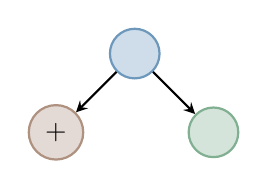
\begin{tikzpicture}[auto]

%
% Styles
%
\tikzstyle{symbol} = [circle,draw=mydarkred!60,fill=mydarkred!20,thick]
\tikzstyle{term}   = [circle,draw=oproverblue!60,fill=oproverblue!20,thick, text width=10pt]
\tikzstyle{list}   = [circle,draw=mydarkgreen!60,fill=mydarkgreen!20,thick, text width=10pt]

\tikzstyle{edge}   = [->,>=stealth,thick]

\node[symbol] (x) at ( -1, 0)  {$+$};
\node[term]   (y) at (  0, 1)  {};
\node[list]   (z) at (  1, 0)  {};

\draw[edge] (y) -- (x);
\draw[edge] (y) -- (z);

\end{tikzpicture}
 
      \end{center}
    \end{column}

    \begin{column}{.45\textwidth}
      \begin{center}
      List
      \bigskip\\
      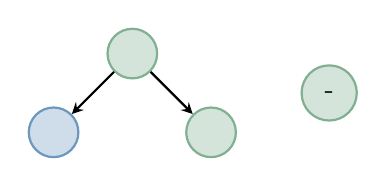
\begin{tikzpicture}[auto]

%
% Styles
%
\tikzstyle{symbol} = [circle,draw=mydarkred!60,fill=mydarkred!20,thick]
\tikzstyle{term}   = [circle,draw=oproverblue!60,fill=oproverblue!20,thick, text width=10pt]
\tikzstyle{list}   = [circle,draw=mydarkgreen!60,fill=mydarkgreen!20,thick, text width=10pt, align=center]

\tikzstyle{edge}   = [->,>=stealth,thick]

\node[term]   (x)   at ( -1, 0)   {};
\node[list]   (y)   at (  0, 1)   {};
\node[list]   (nil) at (  2.5, 0.5) {-};
\node[list]   (z)   at (  1, 0)   {};

\draw[edge] (y) -- (x);
\draw[edge] (y) -- (z);

\end{tikzpicture}
 
      \end{center}
    \end{column}

  \end{columns}

  \vfill\pause

  \begin{columns}

    \begin{column}{.5\textwidth}
      E.g. the term $x \leq y$ is represented as
      \bigskip\\
      If \verb|e| is the Enode for $x \leq y$, we retrieve
      the Enode for \verb|x| with\\
      \verb|Enode * lhs = e->get1st( )|
      \medskip\\
      and the Enode for \verb|y| with\\
      \verb|Enode * rhs = e->get2nd( )|
    \end{column}

    \begin{column}{.5\textwidth}

      \begin{center}
        \scalebox{.7}{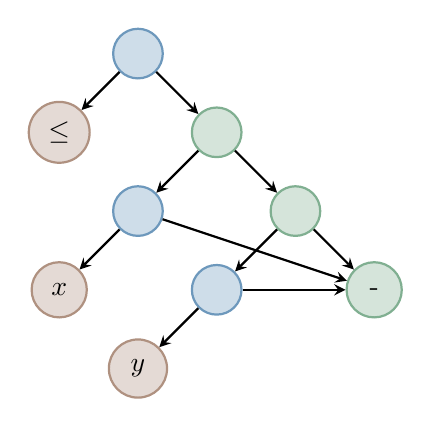
\begin{tikzpicture}[auto]

%
% Styles
%
\tikzstyle{symbol} = [circle,draw=mydarkred!60,fill=mydarkred!20,thick, text width=10pt, align=center]
\tikzstyle{term}   = [circle,draw=oproverblue!60,fill=oproverblue!20,thick, text width=10pt]
\tikzstyle{list}   = [circle,draw=mydarkgreen!60,fill=mydarkgreen!20,thick, text width=10pt, align=center]

\tikzstyle{edge}   = [->,>=stealth,thick]

\node[symbol]   (s1) at (  0,  0)  {$\leq$};
\node[symbol]   (s2) at (  0, -2)  {$x$};
\node[symbol]   (s3) at (  1, -3)  {$y$};
\node[term]     (t2) at (  1, -1)  {};
\node[term]     (t3) at (  2, -2)  {};
\node[term]     (t)  at (  1,  1)  {};
\node[list]     (l2) at (  2,  0)  {};
\node[list]     (l1) at (  3, -1)  {};
\node[list]     (l0) at (  4, -2)  {-};

\draw[edge]  (t) -- (s1);
\draw[edge]  (t) -- (l2);
\draw[edge] (l2) -- (t2);
\draw[edge] (l2) -- (l1);
\draw[edge] (l1) -- (t3);
\draw[edge] (l1) -- (l0);
\draw[edge] (t2) -- (l0);
\draw[edge] (t3) -- (l0);
\draw[edge] (t2) -- (s2);
\draw[edge] (t3) -- (s3);

\end{tikzpicture}
}
      \end{center}

    \end{column}

  \end{columns}

\end{frame}

\begin{frame}[fragile]
  \frametitle{Phase 3 - Implementing the solver}
  \framesubtitle{Playing with the Enodes}

  The polarity of an Enode can be retrieved with
  \begin{center}
  \verb|lbool sign = e->getPolarity( );|
  \end{center}
  and it could be \verb|l_True| or \verb|l_False|
  \vfill
  An Enode \verb|e| can be simply printed with
  \begin{center}
  \verb|cerr << "printing enode: " << e << endl;|
  \end{center}

\end{frame}

\begin{frame}[fragile]
  \frametitle{Phase 3 - Implementing the solver}

  A set of constraints is unsatisfiable iff there is a cycle 
  $$x \leq y,\ y \leq z,\ \ldots,\ w \leq x$$  
  \vfill
  A model is therefore is any ``acyclic'' set of constraints
  \vfill

  \begin{columns}

    \begin{column}{.3\textwidth}

      \begin{overlayarea}{.3\textwidth}{40pt}

	$x \leq y$ \\
	$y \leq z$ \\
	$z \leq x$

      \end{overlayarea}
      
    \end{column}
    
    \begin{column}{.4\textwidth}

      \begin{overlayarea}{.4\textwidth}{40pt}
      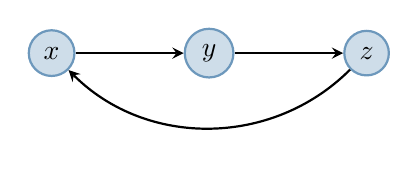
\begin{tikzpicture}[auto]

%
% Styles
%
\tikzstyle{vertex} = [circle,draw=oproverblue!60,fill=oproverblue!20,thick]
\tikzstyle{edge}   = [->,>=stealth,thick]

\node[vertex] (x) at ( 0, 0)  {$x$};
\node[vertex] (y) at ( 2, 0)  {$y$};
\node[vertex] (z) at ( 4, 0)  {$z$};

\draw[edge] (x) -- (y);
\draw[edge] (y) -- (z);
\draw[edge] (z) to [out=225,in=-45] (x);

\end{tikzpicture}

      \end{overlayarea}
      
    \end{column}

    \begin{column}{.2\textwidth}

      unsat

    \end{column}

  \end{columns}

  \vfill
  Therefore we need to

  \begin{enumerate}

    \item Represent the graph from the received constraints

    \item Check if the graph contains a cycle

  \end{enumerate}

\end{frame}

\begin{frame}[fragile]
  \frametitle{Phase 3 - Implementing the solver}
  \framesubtitle{Representing the graph}

  We represent the graph with {\bf adjacency lists}, i.e., every node (variable) is
  assigned to a list of outgoing edges
  \vfill
  We use STL to make the following data structure
  \begin{verbatim}
    map< Enode *, vector< Enode * > > adj_list;
  \end{verbatim}
  that we declare as private attribute in \verb|SOSolver.h|, so that
  it will be accessible everywhere in the class
  \vfill
  When we receive a new constraint with \verb|assertLit|, we update
  \verb|adj_list| with 
  \begin{verbatim}
    adj_list[ from ].push_back( e );
  \end{verbatim}

\end{frame}

\begin{frame}[fragile]
  \frametitle{Phase 3 - Implementing the solver}
  \framesubtitle{Checking for a cycle}

  \scriptsize

  When \verb|check| is called we have to see if there is a cycle in the current graph
  \vfill
  We use a simple depth-first search using the following high-level recursive function:
  \vfill
  \begin{tabbing}
  sd \= sd \= sd \= asd \kill
  \> Input: a node ``from'' \\
  \> Output: $true$ iff a cycle containing ``from'' is found \\
  \> \\
  1 \> function findCycle( Enode * from ) \\
  \\
  2 \> \> if ( ``from was seen before'' ) return $true$ \\ 
  \\
  3 \> \> for each ``from $\leq$ y'' in adj\_list of from \\ 
  4 \> \> \> res = findCycle( y ) \\
  5 \> \> \> if ( res == $true$ ) return $true$ \\
  \\
  6 \> \> return $false$
  \end{tabbing}

\end{frame}

\begin{frame}[fragile]
  \frametitle{Phase 3 - Implementing the solver}
  \framesubtitle{Checking for a cycle}

  \scriptsize

  In SOSolver.C

  \begin{verbatim}
  ...
  bool SOSolver::findCycle( Enode * from )
  {
    if ( seen.find( from ) != seen.end( ) )
      return true;
    
    seen.insert( from );
    vector< Enode * > & adj_list_from = adj_list[ from ];
    
    for ( size_t i = 0 ; i < adj_list_from.size( ) ; i ++ )
    {
      const bool cycle_found = findCycle( adj_list_from[ i ]->get2nd( ) );
      if ( cycle_found ) 
        return true;
    }
    
    seen.erase( from );
    return false;
  }
  ...
  \end{verbatim}

\end{frame}

\begin{frame}[fragile]
  \frametitle{Phase 3 - Implementing the solver}
  \framesubtitle{Checking for a cycle}

  \scriptsize

  In SOSolver.C

  \begin{verbatim}
  bool SOSolver::check( bool complete )    
  { 
    for ( map< Enode *, vector< Enode * > >::iterator it = adj_list.begin( )
        ; it != adj_list.end( )
        ; it ++ )
    {
      seen.clear( );
    
      Enode * from = it->first;
      const bool cycle_found = findCycle( from ); 
    
      if ( cycle_found )
        return false;
    }
    
    return true;
  }
  \end{verbatim}

\end{frame}

\begin{frame}[fragile]
  \frametitle{Phase 3 - Implementing the solver}
  \framesubtitle{Checking for a cycle}

  In SOSolver.h

  \begin{verbatim}
  private:

    bool findCycle ( Enode * );
   
    map< Enode *, vector< Enode * > > adj_list;
    set< Enode * > seen;
  \end{verbatim}

  We can try to compile, and test it with files 
  so\_example\_1.smt2 and so\_example\_2.smt2

\end{frame}

\begin{frame}[fragile]
  \frametitle{Phase 3 - Implementing the solver}
  \framesubtitle{Computing conflicts}

  \scriptsize

  Conflicts can be computed by keeping track of
  the edges that form the last cycle detected 
  \vfill
  We add a \verb|map< Enode *, Enode * > parent_edge|
  map which we use to store the edge used to reach
  a node in the depth-serch traversal
  \vfill
  When during findCycle we discover an already visited
  node, we backward visit the parent\_edge relation
  to retrieve the cycle
  \vfill
  \begin{verbatim}
  void SOSolver::computeExplanation( Enode * from )
  {
    assert( explanation.empty( ) );
    Enode * x = from;
    do
    {
      x = parent_edge[ x ]->get1st( );
      explanation.push_back( parent_edge[ x ] );
    }
    while( x != from );
  }
  \end{verbatim}

\end{frame}

\begin{frame}[fragile]
  \frametitle{Phase 3 - Implementing the solver}
  \framesubtitle{Computing conflicts}

  \scriptsize

  Again in SOSolver.C

  \begin{verbatim}
  void SOSolver::findCycle( Enode * from )
  {
    if ( seen.find( from ) != seen.end( ) )
    {
      computeExplanation( from );
      return true;
    }
    ...
  }
  \end{verbatim}

  \vfill
  Again in SOSolver.h

  \begin{verbatim}
    map< Enode *, Enode * > parent_edge;
  \end{verbatim}

\end{frame}

\begin{frame}[fragile]
  \frametitle{Phase 3 - Implementing the solver}
  \framesubtitle{Incrementality - Backtrackability}

  Last thing we need is to handle incrementality/backtrackability
  \vfill
  For simplicity, solving will not be incremental nor backtrackable in this lecture
  \vfill
  However we still have to keep \verb|adj_list| updated with constraints received/dropped
  \vfill
  For this aim we introduce two more vectors in SOSolver.h

  \begin{verbatim}
  vector< Enode * > used_constr;
  vector< size_t >  backtrack_points;
  \end{verbatim}

  \verb|used_constr| keeps track of the order of constraints received,
  while \verb|backtrack_points| keeps track of the {\bf size} of 
  \verb|used_constr| when a new backtrack point is requested

\end{frame}

\begin{frame}[fragile]
  \frametitle{Phase 3 - Implementing the solver}
  \framesubtitle{Incrementality - Backtrackability}

  \scriptsize

  \begin{verbatim}
  void SOSolver::pushBacktrackPoint ( )
  {
    backtrack_points.push_back( used_constr.size( ) );
  }
  \end{verbatim}

  \begin{verbatim}
  void SOSolver::popBacktrackPoint ( )
  {
    assert( !backtrack_points.empty( ) );
    const size_t new_size = backtrack_points.back( );
    backtrack_points.pop_back( );
    
    while ( new_size < used_constr.size( ) )
    {
      Enode * e = used_constr.back( );
      Enode * from = e->get1st( );
      Enode * to   = e->get2nd( );
      assert( adj_list[ from ].back( ) == e );
      adj_list[ from ].pop_back( );
      used_constr.pop_back( );
    }
  }
  \end{verbatim}

\end{frame}


\begin{frame}
  \frametitle{Exercizes}

  \begin{enumerate}

    \item Show that the \tconflicts generated by the Simplex are minimal

    \vfill
    \item Suppose that $(0,1) \leq x \leq (1,-1)$. Compute the biggest possible value for $\delta$

    \vfill
    \item Find the candidate for pivoting in this row (for simplicity we use normal numbers)
	  $$
	  x_1 = 3 x_2 - 9 x_3 - 7 x_4
	  $$
	  given these bounds $-\infty \leq x_1 \leq 1$, $0 \leq x_2 \leq \infty$, $- \infty \leq x_3 \leq -1$, $1 \leq x_4 \leq 2$
	  and this assignment $\mu = \{ x_1 \mapsto \colone{2}, x_2 \mapsto 0, x_3 \mapsto -1, x_4 \mapsto 1 \}$
    \vfill

    \item Using the row of previous exercize, change the bounds
          so that the only candidate for pivoting becomes $x_2$

    \item Now change the bounds so that no pivoting is possible.
          Compute the conflict

  \end{enumerate}

\end{frame}


\end{document}
